\chapterimage{metodo.jpg} 
\chapter{Metodología}
%%Aquí se define la metodología que se va a utilizar

\begin{figure}[th!]
	\centering
	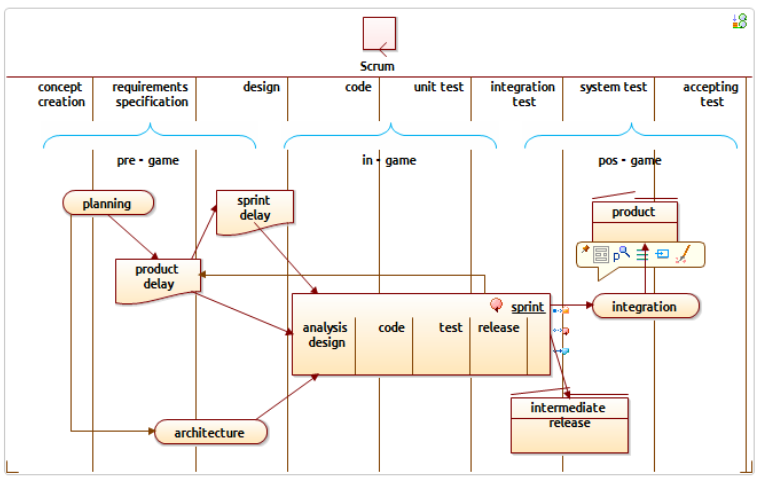
\includegraphics[width=0.6\linewidth]{Scrum}
    \caption{Metodología Scrum}
	\label{fig:Scrum}
\end{figure}
\section{Introducción}
Durante mucho tiempo se buscaron procesos  que se pudieran aplicar en casi cualquier proyecto de desarrollo, los cuales garantizaran la calidad del software y optimizara los tiempos de trabajo, para de esta forma garantizar un producto final de calidad entregado en el plazo de tiempo establecido. El no contar con un proceso de desarrollo puede verse reflejado en el tiempo de producción, ya que este puede ser mucho mayor que el esperado, esto implica igualmente un aumento en los costos.
Las metodologías de desarrollo ágiles surgen debido a la necesidad de generar entregas en el menor tiempo posible, teniendo como prioridad el contacto con el cliente, y la satisfacción de este, para adaptarse de forma rápida al cambio de los requerimientos, del mercado  y a las tecnologías nuevas que se desarrollan, sin dejar de lado la calidad del software en cada entrega.
\newpage
\section{Scrum}
El scrum es un marco de referencia para el desarrollo de software que va de la mano con los principios del manifiesto ágil, el cual busca servir como guía para los procesos de establecer los requerimientos, análisis, diseño, avances y entregas.
Este método fue desarrollado por Jeff Sutherland y su equipo de desarrollo en el año 1990. En años más recientes Schwaber y Beedle han desarrollado más el método Scrum.\cite{Pressman_2010}
En esta metodología el trabajo es dividido en sprints, que por lo general duran dos semanas, pero puede variar dependiendo del tiempo disponible, durante cada sprint se realizan reuniones diarias de por lo general 15 minutos de duración, los cuales sirven para actualizar los avances, informar de los obstáculos que se han presentado y planear lo que se hará hasta la próxima reunión. Esto funciona como estrategia para garantizar que los procesos planteados para el sprint se cumplan.
\newline
\newline
En cada Sprint se incluyen los requerimientos más importantes, los que se van a desarrollar en esa iteración, los cuales están ordenados en una pila de trabajo, en donde las prioridades se encuentran en la parte superior de la pila. Se discute un plan para la realización de los requerimientos, listando las tareas necesarias para estos. Al final de cada sprint se espera que las funcionalidades que entraron estén terminadas y listas para ser presentadas al cliente, se hace también una retrospectiva para evaluar la forma de trabajar del equipo, todos los aspectos a mejorar para la próxima iteración.
\newline
\newline
En la metodología Scrum se cuenta con distintos actores,los cuales tienen un papel importante en el desarrollo del producto:
\newline
\begin{itemize}
	\item Dueño del producto: Esta persona define los requerimientos del producto y es el único que dado el caso puede cambiarlos.
	\item Equipo de trabajo: Son grupos multidisciplinarios y auto-organizados, que trabajan en el desarrollo del producto.
	\item Scrum master o Facilitador: Es una persona externa, preferiblemente, a los grupos de trabajo, la cual dirige los encuentros diarios, ayuda a dar solución a los diferentes problemas que se puedan presentar y evalúa el progreso que tiene cada persona con el fin de conseguir los objetivos de cada iteración.
\end{itemize} 
\newpage
\section{Ventajas y Desventajas}

\subsection{Ventajas}

\begin{itemize}
\item A diferencia de las metodologías tradicionales, el scrum nos permite un desarrollo del proyecto dinámico y ágil, es decir podemos estar enviando entregables al cliente y al mismo tiempo, si es necesario, modificarlo de acuerdo a nuevas especificaciones o necesidades.

\item Permite una mayor eficiencia por parte de cada persona perteneciente al proyecto, esto debido a que cada quien sabe cual es su tarea, es decir requiere de un gran orden para ser aplicado.

\item Da un rol mas incluyente al cliente y a los desarrolladores del software, esto debido a que es más frecuente las pruebas y entregables del software para el perfeccionamiento del mismo.

\item Permite una planeación detallada de los objetivos a alcanzar, por lo que los imprevistos son menos probables a la hora de la codificación. 
\end{itemize} 
\subsection{Desventajas}

\begin{itemize}
\item El hecho de que se le de un rol tan importante a cada miembro del proyecto, puede traer el inconveniente de que alguno de ellos por distintas causas, no pueda cumplir con su tarea, esto implicaría el retraso en el desarrollo o la sobrecarga de trabajo de otros miembros.

\item Muchas veces se puede presentar que no se cumpla con las fechas estipuladas para los entregables, o simplemente que a la hora de presentarlos no se haya logrado un avance significativo.

\item Es necesario excesivas reuniones entre equipo desarrollador y cliente, todo para la verificación y seguimiento del proyecto, ante esto se pueden presentar problemas de disponibilidad.

\item Un error en Pila de Trabajo significaría la carencia de alguna parte esencial del producto, o por el contrario un desperdicio de tiempo y recursos.
\end{itemize} 
\newpage
\section{Cronograma}
\begin{figure}[th!]
	\centering
	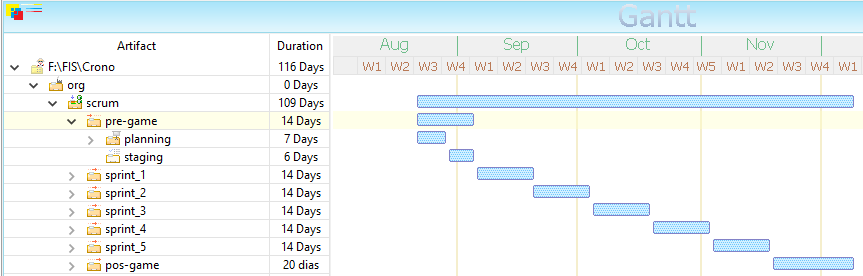
\includegraphics[width=1\linewidth]{Cronograma}
    \caption{Cronograma de la metodología de scrum}
	\label{fig:Cronograma}
\end{figure}